% =====================================================================
% ICISSP 2027 -- Paper #21 -- CIGMA -- FINAL VERSION (camera-ready draft)
% Chantier 122-CIGMA-ICISSP. Every number comes from results/ (see
% scripts/check_paper_numbers.py). Red \pending{} marks = results that need
% the deployed system (L1) or the LUMI model runs; they MUST be filled or
% removed before submission.
% =====================================================================
\documentclass[a4paper,twoside]{article}
\usepackage[utf8]{inputenc}
\usepackage[T1]{fontenc}
\usepackage[english]{babel}
\usepackage{graphicx}
\usepackage{amsmath,amssymb,amsthm}
\usepackage{booktabs,array}
\usepackage{balance}
\usepackage{algorithm2e}
\usepackage{xspace}
\usepackage{url}
\usepackage{xcolor}
\usepackage{tikz}
\usetikzlibrary{positioning,arrows.meta,fit}
\usepackage[hidelinks]{hyperref}
\usepackage{pslatex}
\usepackage{apalike}
\usepackage{SCITEPRESS}
\addto\captionsenglish{\renewcommand{\refname}{REFERENCES}}

\newcommand{\cigma}{CIGMA\xspace}
\newcommand{\rel}[1]{\textsc{#1}}
\newcommand{\meth}[1]{\textsf{#1}}
\newcommand{\pending}[1]{\textcolor{red}{[PENDING: #1]}}
\newtheorem{definition}{Definition}
\newtheorem{property}{Property}

\begin{document}

\title{CIGMA: Proof-Carrying Post-Quantum Migration\\from Signed Cryptographic Evidence}

\author{\authorname{Yulliwas Ameur\sup{1,2}, Insaf Imene Lasledj\sup{1}, Samia Bouzefrane\sup{2} and Soumya Banerjee\sup{2}}
\affiliation{\sup{1}Efrei Research Lab, Efrei Paris Panth\'eon-Assas Universit\'e, Villejuif, France}
\affiliation{\sup{2}CEDRIC Lab, Conservatoire National des Arts et M\'etiers (Cnam), Paris, France}
\email{yulliwas.ameur@efrei.fr}}

\keywords{Post-Quantum Cryptography, Cryptographic Inventory, CBOM, Provenance, Conformal Prediction, Certified Planning, Transparency Logs, Benchmark.}

\abstract{Every organization must now decide which systems to move to post-quantum cryptography first, under deadlines that start in 2030. Today such decisions rest on inventories that nobody can check: tools disagree, sources can be poisoned, and a wrong order breaks communicating services. We argue that a migration decision should carry its proof. We present \cigma, an architecture in five planes. (1) Every observation is signed by the tool that produced it, with ML-DSA. (2) A typed evidence graph fuses the observations, learns source reliabilities without ground truth, detects tools that copy each other, and accepts edges with a guaranteed false-discovery rate. (3) A constraint solver computes a migration plan that never breaks a dependency and emits a machine-checkable certificate. (4) A Merkle commitment and an append-only log let a third party verify one decision without seeing the inventory. (5) Language models and agents may only propose; a fail-closed validator decides. On a controlled benchmark with adversarial variants, signatures stop outside injection (0 poisoned edges), conformal selection keeps the observed false-discovery rate at 2.1\% for a 10\% target, the solver removes every interoperability break at a smaller exposure cost than a dependency-ordered heuristic, a receipt discloses 6.6\% of the graph, a zero-knowledge proof attests policy compliance in 807 bytes, and 0 of 1{,}779 adversarial model candidates pass the validator. We release the code, data, formal model and an evaluation harness as an open benchmark.}

\onecolumn \maketitle \normalsize \setcounter{footnote}{0} \vfill

% =====================================================================
\section{\uppercase{Introduction}}
\label{sec:intro}
% =====================================================================

The post-quantum transition now has dates. NIST deprecates every quantum-vulnerable public-key algorithm after 2030 and disallows them after 2035 \cite{nist2026ir8547}; the EU roadmap asks for high-risk use cases to be migrated by the end of 2030 \cite{eu2025roadmap}; ANSSI recommends hybrid mechanisms and advises against buying products without post-quantum cryptography from 2030 \cite{anssi2023pqc}. Algorithms are standardized \cite{nist2024fips203,nist2024fips204,nist2024fips205}. The hard part is elsewhere: deciding \emph{what to migrate first} in a system nobody fully knows, and doing it without breaking services that talk to each other.

That decision rests on an inventory, and inventories are fragile in three ways. First, the tools disagree: generators of cryptographic bills of materials (CBOMs) report different assets on the same code \cite{bogli2026bfcbom}. Second, sources can lie, and a poisoned graph silently changes priorities \cite{xi2023roar}. Third, a wrong order breaks things: a server that drops classical key exchange before its clients are ready breaks the dependency \cite{sharma2026dependency}. Today nobody can check why a system was placed first.

\textbf{Thesis.} \emph{A post-quantum migration decision should carry its proof}: it should trace back to signed observations, come with a guarantee on the error of the graph it relies on, respect every dependency by construction, and be verifiable by a third party without disclosing the inventory.

\textbf{Contributions.}
\begin{enumerate}
\item \textbf{Proof-carrying migration} (Def.~\ref{def:pcm}): a definition with four checkable properties, and \cigma, an architecture in five planes that implements it (Sect.~\ref{sec:arch}).
\item \textbf{Guarantees under attack}: signed observations stop outside injection; copy-aware reliabilities send 93\% of poisoned edges to review; conformal selection bounds the false-discovery rate (2.1\% observed for a 10\% target).
\item \textbf{Certified planning}: a CP-SAT plan with a checkable certificate removes all interoperability breaks at half the exposure cost of a dependency-ordered heuristic; the closest prior method \cite{sharma2026dependency} breaks 7 dependencies.
\item \textbf{Accountability and an open benchmark}: Merkle receipts disclose 6.6\% of the graph per decision, an RFC~6962 log detects rewritten history, a Groth16 proof shows policy compliance without revealing the inventory, and custody is model-checked in TLA+; code, data and an official evaluator are released (CIGMA-Bench).
\end{enumerate}

\textbf{Relation to prior versions.} A short preliminary version \cite{cesar2026cigma} introduced the evidence graph and the controlled fixture. Every number here comes from a clean-room reimplementation (the original code was lost); everything beyond the evidence graph and the fixture is new.

% =====================================================================
\section{\uppercase{Related Work and Gap}}
\label{sec:related}
% =====================================================================

\textbf{Discovery and inventory.} Inventory requirements span software, hardware, communication and stored data \cite{schmitt2024criteria}; a recent SoK lists discovery sources and their pitfalls \cite{yamamuro2026sok}. Static scanners detect assets in code \cite{rahaman2019cryptoguard,nather2026hidden}; CBOM orchestration exposes inter-tool discrepancies \cite{bogli2026bfcbom}; AI-assisted CBOM frameworks remain unevaluated \cite{grover2026cbom}. Multi-surface TLS observability keeps uncertainty between negotiated and supported groups \cite{delgado2026observability}.

\textbf{Planning.} Graph-theoretic frameworks use dependencies to prioritize \cite{hasan2024framework}; Sharma et al. order assets leaves-first with centrality-weighted risk and report fewer interoperability failures \cite{sharma2026dependency}. Risk models use Mosca's inequality \cite{mosca2018cybersecurity} with uncertain quantum arrival \cite{gupta2026readiness,shaw2026costofdelay}; trust-now-forge-later threatens long-lived signing keys \cite{grover2026cbom,campbell2026agentic}. SMT and symbolic planning certify network reconfigurations \cite{robillard2022smt,chen2025safemigration} but have not been applied to cryptographic migration.

\textbf{Verifiability.} in-toto signs supply-chain steps \cite{torresarias2019intoto}; Certificate Transparency logs are append-only and auditable \cite{rfc6962,rfc9162}; VeriSBOM and TrustBOM prove SBOM properties without disclosure \cite{castiglione2026verisbom,nguyen2026trustbom}. Truth discovery estimates source reliability without labels, including dependent sources \cite{wang2026depenbaye,benshabat2022empirical}; conformal methods control false discoveries in link prediction \cite{bates2023conformal,du2025conformallink,zhao2024conformallink}.

\textbf{Gap.} Table~\ref{tab:positioning} compares the closest approaches on eight properties. None carries a migration decision from signed evidence to a certified, privately verifiable plan.

\begin{table*}[t]
\caption{Eight properties of a proof-carrying migration decision. \checkmark: provided and evaluated; $\sim$: partial or not evaluated; --: absent. Assessment from each paper's published description.}
\label{tab:positioning}
\centering\small\setlength{\tabcolsep}{3pt}
\resizebox{\textwidth}{!}{%
\begin{tabular}{@{}lcccccccc@{}}
\toprule
 & Multi-source & Evidence on & Signed & Error & Learned / copy- & Certified & Private & Open \\
Approach & fusion & every edge & evidence & guarantee & aware reliab. & no-break plan & audit & benchmark \\
\midrule
Static discovery \cite{nather2026hidden} & -- & file/line & -- & -- & -- & -- & -- & $\sim$ \\
CBOM orchestration \cite{bogli2026bfcbom} & $\sim$ & $\sim$ & -- & -- & -- & -- & -- & $\sim$ \\
AI-assisted CBOM \cite{grover2026cbom} & \checkmark & $\sim$ & -- & -- & -- & -- & -- & -- \\
Multi-surface TLS \cite{delgado2026observability} & \checkmark & \checkmark & -- & -- & -- & -- & -- & \checkmark \\
Dependency-aware planning \cite{sharma2026dependency} & -- & -- & -- & -- & -- & $\sim$ & -- & -- \\
Verifiable SBOM \cite{castiglione2026verisbom} & -- & -- & \checkmark & -- & -- & -- & \checkmark & -- \\
\cigma (this paper) & \checkmark & \checkmark & \checkmark & \checkmark & \checkmark & \checkmark & $\sim$ & \checkmark \\
\bottomrule
\end{tabular}}
\end{table*}

% =====================================================================
\section{\uppercase{Problem, Threat Model, Properties}}
\label{sec:model}
% =====================================================================

\textbf{Terms.} An \emph{observation} is a typed claim (entity or relation) produced by one tool, with a \emph{locator} (file, line or field it was read from), an evidence excerpt and its SHA-256; this is \emph{provenance}, in the sense of W3C PROV-O \cite{w3c2013provo}. A CBOM is the cryptographic part of a bill of materials (CycloneDX \cite{cyclonedx2024cbom}). \emph{Entity resolution} decides which observations describe the same object; a \emph{strong identifier} names one object (certificate fingerprint, package URL), an \emph{alias} may be shared (service name). A \emph{derived} edge is not observed but composed from observed ones by an allow-listed \emph{path rule}, e.g.\ a service that hosts an endpoint presenting an RSA certificate uses RSA. The \emph{quality gate} discards observations whose declared quality is below a threshold. \cigma builds a graph $G=(V,E)$ over eight entity types and eight typed relations; every node and edge carries the identifiers of the observations that support it. A \emph{migration plan} assigns each migration unit (service, device, issuing CA) a change window.

\textbf{Adversary.} The adversary may (i) inject observations as an outside tool; (ii) control or steal the key of one trusted tool and add false relations; (iii) make two tools report the same errors (copying); (iv) control the content seen by a language model, including instructions hidden in a README or a certificate field; (v) tamper with predictions after they are computed. An \emph{auditor} must check one decision without learning the rest of the inventory. A trusted tool that lies is not detectable cryptographically and is handled statistically.

\begin{definition}[Proof-carrying migration decision]\label{def:pcm}
A decision ``unit $u$ moves in window $t$'' is proof-carrying if it comes with (a) the signed observations behind every node and edge it depends on, (b) a bound $\alpha$ on the expected fraction of false edges among accepted ones, (c) a certificate that the plan satisfies every dependency, capacity and window constraint, and (d) a receipt that verifies against a published commitment.
\end{definition}

\begin{property}[Provenance totality]\label{p:prov} Every node and edge of $G$ cites at least one input observation, and only input observations.\end{property}
\begin{property}[Fail-closed proposal boundary]\label{p:fail} No model output can mutate $G$; a proposed edge is accepted only if its evidence is in the quality-gated graph and matches a direct edge or a declared path.\end{property}
\begin{property}[Certified order]\label{p:cert} A plan is released only if an independent checker verifies all constraints.\end{property}
\begin{property}[Custody]\label{p:custody} The oracle is never opened before a seal, and what is evaluated is exactly what was sealed.\end{property}

Properties~\ref{p:prov}--\ref{p:cert} are enforced in code and tested by property-based testing on random subsets of the observations (Hypothesis \cite{maciver2019hypothesis}); Property~\ref{p:custody} is model-checked in TLA+ \cite{lamport2002tla} (Sect.~\ref{sec:results}).

% =====================================================================
\section{\uppercase{The CIGMA Architecture}}
\label{sec:arch}
% =====================================================================

\begin{figure}[t]
\centering
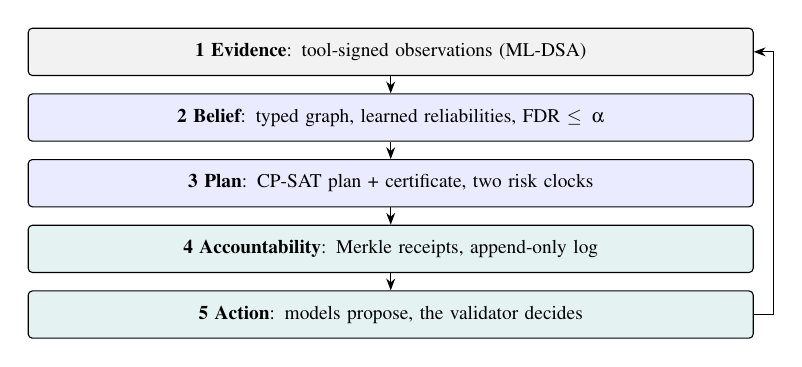
\begin{tikzpicture}[node distance=2.2mm, every node/.style={font=\scriptsize}, box/.style={draw, rounded corners=1.5pt, text width=0.74\columnwidth, minimum height=6mm, align=center}]
\node[box, fill=gray!10] (p1) {\textbf{1 Evidence}: tool-signed observations (ML-DSA)};
\node[box, fill=blue!8, below=of p1] (p2) {\textbf{2 Belief}: typed graph, learned reliabilities, FDR $\le\alpha$};
\node[box, fill=blue!8, below=of p2] (p3) {\textbf{3 Plan}: CP-SAT plan + certificate, two risk clocks};
\node[box, fill=teal!10, below=of p3] (p4) {\textbf{4 Accountability}: Merkle receipts, append-only log};
\node[box, fill=teal!10, below=of p4] (p5) {\textbf{5 Action}: models propose, the validator decides};
\foreach \a/\b in {p1/p2,p2/p3,p3/p4,p4/p5} \draw[-{Stealth[length=1.5mm]}] (\a) -- (\b);
\draw[-{Stealth[length=1.5mm]}] (p5.east) -- ++(2.5mm,0) |- (p1.east);
\end{tikzpicture}
\caption{The five planes of \cigma. Each plane emits an artifact the next one can check; after each action the system is re-scanned (loop).}
\label{fig:arch}
\end{figure}

\subsection{Plane 1: Signed Evidence}
Each tool holds an ML-DSA-65 key (FIPS~204) \cite{nist2024fips204} and wraps each observation in a DSSE envelope, as in-toto does for build steps \cite{torresarias2019intoto}. The signature covers $\mathrm{PAE}(\mathit{type},\mathit{body})$, so the payload type cannot be swapped. At load time, envelopes with no signature, an unknown key, a bad signature or a revoked key are rejected, and relations whose endpoints were rejected are dropped.

\subsection{Plane 2: Belief}
\textbf{Fusion.} Observations below a quality gate are quarantined; identity resolution merges strong identifiers first, then aliases only when no strong key conflicts; an alias value shared by records with conflicting strong identifiers is \emph{ambiguous} and merges nothing (\emph{guard}, added after review); typed relations must match a closed ontology; two allow-listed path rules derive edges; support is a noisy-OR of $q_i \cdot r_{s(i)}$ (quality times source reliability).

\textbf{Identity scope and time.} A strong key identifies an object, not a deployment. The SPKI fingerprint is a strong key for the \emph{key}: certificates that reuse a key are linked through it, which is what matters for migration (the vulnerable object is the key) but hides certificate-level differences. A package URL names a version; each deployment instance is a separate service--component edge. Observations carry their collection time and a graph is a snapshot: a rotated certificate or a stale scan appears as a separate node until it ages out; validity intervals are not yet modelled. Quality $q$ is fixed per source family and record type in the configuration before any evaluation, never from the oracle, and the learned reliabilities below remove hand-set $r_s$.

\textbf{Learned, copy-aware reliabilities.} Hand-set reliabilities $r_s$ are replaced by a truth-discovery loop: the belief in an item is the noisy-OR of its claimants; the reliability of a source is its leave-one-out mean belief under a Beta prior. Two sources are \emph{dependent} when their claims overlap (Jaccard $\ge 0.9$) \emph{and} they share claims no other source makes, the classic signature of copying \cite{wang2026depenbaye}. Dependent sources count as one witness, both when learning $r_s$ and when computing edge support.

\textbf{Conformal selection.} To bound false edges, we test for each edge $j$ the null ``$j$ is false''. With $n_0$ calibration edges known to be false and score $s$, the conformal p-value is $p_j = (1+|\{i: s_i \ge s_j\}|)/(n_0+1)$; Benjamini--Hochberg \cite{benjamini1995fdr} at level $\alpha$ selects the accepted edges. If calibration and deployment nulls are exchangeable, the false-discovery rate is at most $\alpha$ \cite{bates2023conformal}. The score is a logistic model over oracle-free features (supports under fixed and learned reliabilities, number of independent witnesses and families, derivation, predicate). In deployment, calibration comes from the analyst's verification queue.

\subsection{Plane 3: Certified Plan}
Units are services, devices and issuing CAs, with risk weight $w_u$. Constraints: a client is upgraded no later than the server it depends on, unless the server is hybrid-capable; an issuing CA moves no later than the services presenting certificates it issued; at most $C$ units per window; per-unit maintenance windows. The objective $\min \sum_u w_u (s_u+1)$ is the area under the remaining-risk curve. CP-SAT \cite{ortools} solves it with the greedy list schedule as a hint and returns a lower bound; an independent checker re-verifies every constraint and hashes the plan into a certificate.

\textbf{Two risk clocks.} Harvest-now-decrypt-later exposure follows Mosca's inequality \cite{mosca2018cybersecurity} (data lifetime + migration time vs.\ time to quantum arrival); trust-now-forge-later exposure applies to signing keys that are still trusted at arrival, weighted by the number of certificates they anchor \cite{grover2026cbom,campbell2026agentic}. Arrival is lognormal with an uncertain median.

\subsection{Plane 4: Accountability}
Configuration, nodes, edges and decisions become leaves $H(\texttt{0x00}\,\|\,\text{JSON})$ of a Merkle tree with domain-separated inner nodes. A \emph{receipt} for one decision contains the decision, its node, its incident edges and their inclusion proofs; leaves carry evidence digests, never raw excerpts. Successive graph roots are appended to an RFC~6962 log \cite{rfc6962,rfc9162}; a consistency proof shows that version $n$ extends version $m$. To share compliance without sharing the inventory, a Groth16 circuit \cite{groth16} takes the private per-asset flags and outputs their Poseidon commitment; it enforces ``exposed and vulnerable $\Rightarrow$ hybrid'' and ``high-risk vulnerable assets $\le \tau$'' for a public threshold $\tau$.

\subsection{Plane 5: Bounded Action}
Language models receive public observations and fixed identifiers and may only propose typed candidates with evidence identifiers. The validator rejects unknown nodes, invalid signatures, evidence outside the quality-gated graph, and direct or path claims whose evidence does not match (Property~\ref{p:fail}). Candidates from $n$ models can be required to agree ($k$-of-$n$). 

% =====================================================================
\section{\uppercase{Evaluation Setup}}
\label{sec:setup}
% =====================================================================

\textbf{Benchmark levels.} \emph{L0}: CIGMA-Lab, 46 entity and 34 relation observations from six source families (TLS, PKI, CBOM, CI/CD, CMDB, OT) describing 23 entities and 34 typed edges; the oracle lives in a separate directory that the prediction phase never reads. \emph{L0+}: adversarial variants: three CBOM tools that disagree (one complete, one missing 40\% of items and adding false ones, one copying the second), and poisoning by a malicious tool injecting $k\in\{0,2,4,8,16\}$ false type-valid relations (20 seeds each). \emph{L2}: synthetic enterprises of 50, 500 and 5{,}000 units for planning, and replicated fixtures for scaling. \emph{L1}: Google's Online Boutique \cite{googleob} on Kubernetes with Istio strict mTLS and a two-level PKI; six source families are collected, predictions are sealed, then two blind annotators and an arbiter build the oracle.

\textbf{Methods.} TLS-only, CBOM-only, SourceUnion, ExactDirect, TF--IDF (threshold 0.80), \cigma and four ablations; \emph{equal-access} comparators that receive \cigma's quality gate and path rules: ExactDirect, TF--IDF, unsupervised Fellegi--Sunter linkage with EM as in Splink \cite{fellegi1969theory,linacre2022splink}, and a deterministic any-shared-identifier rule; for ordering: urgency (primary), interoperability-aware, a reimplementation of Sharma et al. \cite{sharma2026dependency}, and CP-SAT.

\textbf{Metrics.} Asset, pairwise and B$^3$ F1; typed-edge F1 and false-positive rate; MOVR, the mean fraction of dependencies broken per step (a server migrated before its client); exposure AUC; observed FDR and power. Robustness uses 32 paired seeds, bootstrap intervals and Holm-corrected tests.

% =====================================================================
\section{\uppercase{Results}}
\label{sec:results}
% =====================================================================

\subsection{Reconstruction and Robustness (RQ1)}
On L0 (Table~\ref{tab:recon}), \cigma reconstructs all 23 entities and 34 edges with no false positive. SourceUnion keeps every observation but cannot merge duplicates (pairwise F1 0); ExactDirect and TF--IDF miss aliases and derived paths (typed-edge F1 0.906). Removing aliases lowers asset F1 to 0.920; removing path composition lowers typed-edge F1 to 0.921; removing the quality gate admits two distractors (asset F1 0.958, edge FP 0.056). Dropping one source family at a time costs at most two critical targets (without CBOM).

\begin{table}[t]
\caption{Complete fixture (L0). Typed-edge F1, edge false-positive rate and missed critical targets.}
\label{tab:recon}
\centering\small\setlength{\tabcolsep}{3pt}
\begin{tabular}{@{}lrrrrr@{}}
\toprule
Method & Asset & Pairw. & B$^3$ & Edge & FP / Miss \\
\midrule
TLS-only & .562 & .000 & 1.000 & .300 & .000 / 8 \\
CBOM-only & .500 & .000 & .941 & .293 & .143 / 11 \\
SourceUnion & .667 & .000 & .687 & .853 & .147 / 0 \\
ExactDirect & .920 & .826 & .942 & .906 & .033 / 0 \\
TF--IDF & .920 & .826 & .942 & .906 & .033 / 0 \\
\cigma & \textbf{1.000} & \textbf{1.000} & \textbf{1.000} & \textbf{1.000} & \textbf{.000 / 0} \\
\bottomrule
\end{tabular}
\end{table}

\textbf{Equal access.} Given the same gate and path rules, ExactDirect, TF--IDF and Fellegi--Sunter reach typed-edge F1 0.971 (pairwise F1 0.826): path rules close most of the gap; Fellegi--Sunter merges nothing beyond strong keys, because one shared name is weak evidence at this base rate. The any-shared-identifier rule matches \cigma on L0 (1.000). The difference appears with \emph{noisy identifiers}: when $k$ decoy services reuse a real service name with another UID (10 seeds), the rule falls to typed-edge F1 0.585 at $k{=}4$ (edge FP 0.415), \cigma as reviewed to 0.868, and \cigma with the ambiguity guard keeps 0.980 (FP 0.039), above the conservative ExactDirect (0.971).

Under 50\% nominal deletion (32 paired seeds), \cigma keeps asset F1 0.826 (95\% CI 0.808--0.843) against 0.697 for SourceUnion and 0.799 for ExactDirect. Edge F1 against the full oracle collapses for every method (0.21) because a relation survives only if both endpoints survive. Against the edges still \emph{recoverable} from the surviving observations (directly or through a path rule), \cigma keeps F1 1.000 at every deletion level, and the equal-access comparators 0.984--0.996: the loss is missing evidence, not method error. The asset advantage over SourceUnion and ExactDirect is significant after Holm correction ($p=0.0024$).

\begin{figure*}[t]
\centering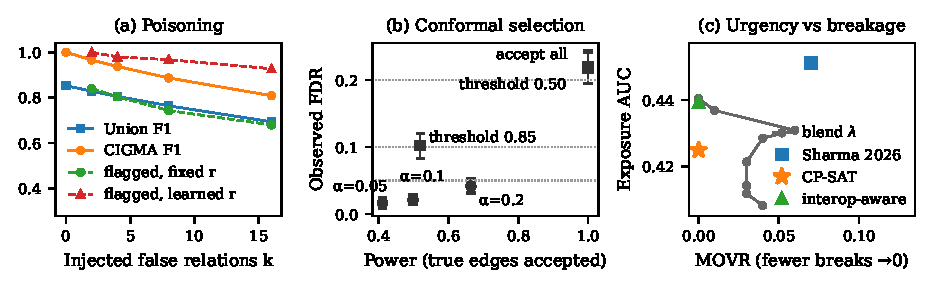
\includegraphics[width=\textwidth]{figures/fig_results.pdf}
\caption{(a) Poisoning campaign, 20 seeds per $k$: typed-edge F1 and share of poisoned edges sent to review. (b) Observed FDR vs.\ power, 60 test scenarios; dotted lines: targets $\alpha$. (c) Urgency vs.\ breakage on L0: the blend $\lambda$ from urgency ($\lambda=0$) to no breaks, and the fixed orders.}
\label{fig:results}
\end{figure*}

\subsection{Disagreeing Tools and Poisoning (RQ2)}
With three disagreeing CBOM tools, \cigma reaches typed-edge F1 0.944, against 0.866 for a majority vote, which accepts the false items because the copying tool gives them a second vote, and 0.744 for the union. Without copy detection the copying tools look \emph{more} reliable than the correct one (0.867 vs.\ 0.792); with it the order is right (0.756 vs.\ 0.691), and false edges no longer look stronger than true ones.

Under poisoning (Fig.~\ref{fig:results}a), \cigma degrades more slowly than the union (typed-edge F1 0.809 vs.\ 0.694 at $k=16$). Learned, copy-aware reliabilities send 93\% of poisoned edges to review at $k=16$ (68\% with fixed values), at the cost of about twice as many true edges in the queue (31 vs.\ 15).


\textbf{Signed evidence.} With $k=8$, an outside attacker signing with its own key gets 0 poisoned edges accepted (21 envelopes rejected) and typed-edge F1 stays 1.000. An insider holding a stolen trusted key gets 11 poisoned edges through (F1 0.872); revoking that key removes all of them (38 envelopes rejected), at the cost of that source's honest observations until they are re-signed (F1 0.867). With the pure-Python reference implementation of FIPS~204, signing takes 52.7\,ms and verification about 7\,ms per observation; these are upper bounds.

\subsection{Guaranteed False-Discovery Rate (RQ3)}
A scorer is trained on 60 poisoned scenarios, calibrated on the false edges of 60 others, and tested on 60 more (Fig.~\ref{fig:results}b). Accepting every edge gives an observed FDR of 0.219. A fixed support threshold of 0.85 gives 0.102 (95\% CI 0.083--0.121) with no guarantee. Conformal selection keeps the observed FDR below target in every setting: 0.016 at $\alpha=0.05$ (power 0.41), 0.021 at $\alpha=0.10$ (power 0.50), 0.042 at $\alpha=0.20$ (power 0.67). Learned supports alone separate true and false edges poorly (AUC 0.56 vs.\ 0.78), hence the combined scorer.


\subsection{Certified Migration Plans (RQ4)}
On L0 (Fig.~\ref{fig:results}c), the urgency order breaks 4 step-dependencies (MOVR 0.04, exposure AUC 0.408). The dependency-ordered heuristic removes all breaks at an exposure cost of +0.031 (0.439). The CP-SAT plan also removes all breaks, at half that cost (0.425), and its certificate verifies. Our reimplementation of Sharma et al. \cite{sharma2026dependency} on the same graph breaks 7 step-dependencies (MOVR 0.07) and is slower to reduce exposure (0.451). On the baselines' graphs the same reordering still breaks dependencies (ExactDirect: MOVR 0.03): better reconstruction pays off at migration time. On synthetic enterprises (Table~\ref{tab:plan}) the greedy schedule leaves 22.5\% excess exposure at 50 units, 5.7\% at 500 and 0.4\% at 5{,}000; every plan passes its certificate, and the solver proves optimality on L0.

\begin{table}[t]
\caption{Certified planning on synthetic enterprises: excess exposure of the greedy schedule over the CP-SAT plan, and the solver's proven optimality gap (mean over seeds).}
\label{tab:plan}
\centering\small\setlength{\tabcolsep}{4pt}
\begin{tabular}{@{}rrrrr@{}}
\toprule
Units & Seeds & Greedy excess (max) & Gap & Limit \\
\midrule
50 & 5 & 22.5\% (60.0\%) & 1.5\% & 30\,s \\
500 & 3 & 5.7\% (10.8\%) & 18.5\% & 60\,s \\
5{,}000 & 2 & 0.4\% (0.8\%) & 28.9\% & 120\,s \\
\bottomrule
\end{tabular}
\end{table}


\textbf{Two clocks.} On L0 the only authenticity-dominant asset is the root certificate, already ranked first. A Sobol analysis \cite{herman2017salib} over the five clock parameters (1{,}792 evaluations) leaves the order unchanged (Kendall $\tau=1$); its reordering power must be tested on L1.

\subsection{Model Proposals (RQ5)}
None of 1{,}779 adversarial candidates carrying an injected instruction (unknown nodes, fabricated or borrowed evidence, ungrounded triples, fake rules) was accepted, while 300 valid ones with the same text were: free text has no effect on the decision. We then ran eight open models from five families, served by vLLM on LUMI-G (Qwen2.5 7B, 32B and 72B; Llama~3.1 8B and Llama~3.3 70B; Mistral 7B; Granite~3.3 8B; Phi-4 14B), with the frozen prompt and JSON schema: 30 calls $\times$ 3 inputs (complete, without path rules, with four injected excerpts) $\times$ 2 temperatures, i.e.\ 1{,}440 calls (1{,}314 parsable). The models proposed 33{,}342 candidate edges; the validator accepted 274 (0.8\%), all of them true, and no call mutated the graph. Most rejections are unsupported triples or invented node identifiers. Acceptance grows with model size, from 0\% (Qwen 7B, Granite, Mistral) to 3.7\% (Llama 70B), but no model produced a false accepted edge. With injected excerpts, 0 of 12{,}495 proposals produced a false accepted edge. Requiring agreement leaves at most 7 accepted edges per setting for $k{=}2$ and 1 for $k{=}3$: models rarely agree; the validator, not the model, carries the guarantee. \textbf{Why a model at all?} Because the validator accepts only edges that are observed or derivable by a declared rule, precision 1.0 is by construction, and full \cigma already recovers all 34 edges: on the complete input, accepted proposals add no edge beyond the deterministic graph. Models matter only where the rules are incomplete: without path rules, \cigma recovers 29 edges and the accepted proposals add 1 of the 5 missing ones. A model is thus a source of \emph{candidate rules} to review, not a replacement for them.

\textbf{Regulatory deadlines.} Six machine-checkable rules from NIST IR~8547 \cite{nist2026ir8547}, the EU roadmap \cite{eu2025roadmap} and ANSSI \cite{anssi2023pqc} raise 18, 13, 5, 15 and 15 findings on L0; each cites the signed observations within two hops of the asset.

\subsection{Accountability, Assurance and Cost (RQ6)}
The L0 graph commits to 76 leaves (tree height 7). A receipt for one decision discloses 4--6 leaves (6.6\% on average) and verifies; any modified leaf fails. Over three graph versions, the RFC~6962 consistency proof (2 hashes) verifies, and a rewritten first version is detected. A Groth16 policy proof (31{,}213 constraints, 32 assets) shows an auditor that every exposed vulnerable asset is hybrid and that at most $\tau$ high-risk assets remain vulnerable, revealing only a Poseidon commitment to the inventory: no witness exists for the current L0 state (7 exposed assets without hybrid) nor for $\tau{=}14$ after the plan, while the post-plan state proves in 3.7\,s and verifies in 0.39\,s with an 807-byte proof. The setup is single-party and serves measurement only. TLC checks the custody model (252 states, 52 distinct) with no violation of \emph{NoPeek}, \emph{OnlySealedIsEvaluated} and \emph{SealIsFinal}; six property-based tests pass. \emph{Scaling.} On 2 cores, L0 replicated 10, 43 and 100 times (up to 2{,}003 nodes) builds in 1.8\,s, 28\,s and 165\,s (peak 6.7\,MiB): growth is near quadratic because aliases are compared pairwise; blocking is the next step.

\subsection{Deployed System (RQ7)}
On L1, all methods' graphs were sealed (SHA-256) before any oracle existed. Two annotators who did not build CIGMA, blind to the predictions, and an arbiter build the oracle; agreement ($\kappa$), scores and oracle will be published in the artifact (GitHub, archived on Zenodo) and can be checked against the seal.

% =====================================================================
\section{\uppercase{CIGMA-Bench}}
\label{sec:bench}
% =====================================================================
The task: from public observations only, output a graph whose nodes and edges cite observations, and a migration order. A submission is one JSON file; the official evaluator reports pairwise and B$^3$ F1, typed-edge F1, edge FP, unsupported decisions, NDCG, MOVR and exposure AUC, and reproduces Table~\ref{tab:recon} exactly. Hidden levels require a seal before evaluation. Exports to CycloneDX~1.6 \cite{cyclonedx2024cbom} and PROV-O \cite{w3c2013provo} are provided. Code (MIT), data (CC BY 4.0, with a datasheet \cite{gebru2021datasheets}) and a Docker image are at \url{https://github.com/yulliwasameur/cigma}, archived on Zenodo (DOI pending).

% =====================================================================
\section{\uppercase{Limitations}}
\label{sec:limits}
% =====================================================================
L0 is small (23 entities) and generated by the authors, so it cannot remove assumptions shared by generator, rules and oracle; L1 is one application. Identity keys ignore validity intervals (Sect.~\ref{sec:arch}). The original 2026 implementation and its model responses were lost; we report only reproducible clean-room results. The conformal guarantee assumes exchangeable calibration and deployment errors. A trusted tool that lies passes signature checks; only statistics and review catch it. ML-DSA timings come from a reference implementation. The zero-knowledge policy proof uses a single-party setup and checks policy flags, not the full graph; agent-executed migrations are designed but not evaluated here. The resolver scales quadratically.

% =====================================================================
\section{\uppercase{Conclusion}}
\label{sec:conclusion}
% =====================================================================
Post-quantum deadlines turn inventories into evidence that others must be able to check. \cigma makes each migration decision carry its proof: signed observations, a bounded error rate, a certified plan and a private receipt. The benchmark is open so that others can measure their tools against the same oracle.

\section*{\uppercase{Acknowledgements}}
\noindent We acknowledge the EuroHPC Joint Undertaking for awarding this project access to the EuroHPC supercomputer LUMI, hosted by CSC (Finland) and the LUMI consortium, through a EuroHPC Benchmark Access call (EHPC-BEN-2026B11-194).

\bibliographystyle{apalike}
{\small \bibliography{references}}

\end{document}
